%This work is licensed under the Creative Commons License Attribution 4.0 International (CC-BY 4.0)
%https://creativecommons.org/licenses/by/4.0/legalcode
\documentclass[rgb]{standalone}
\usepackage{pgfplots}
\definecolor{myorange}{hsb}{0.0833, 1, 0.8}
\definecolor{mygreen}{hsb}{0.3333, 1, 0.8}
\definecolor{myblue}{hsb}{0.5833, 1, 0.8}
\definecolor{mymagenta}{hsb}{0.8333, 1, 0.8}
\begin{document}
	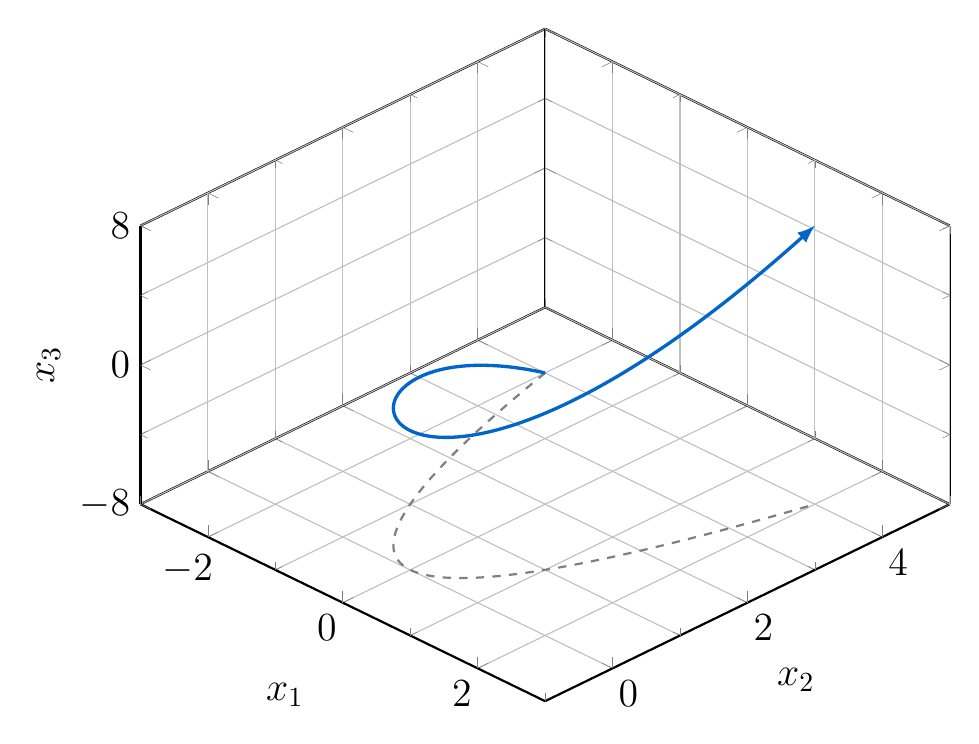
\begin{tikzpicture}[font=\Large]
		\begin{axis}[scale=1.5,thick,grid=both, minor tick num =1,view={45}{45},
			xmin=-3,xmax=3, ymin=-1,ymax=5, zmin=-8, zmax=8, 
			ztick={-8,0,8}, 
			xlabel=$x_1$, ylabel=$x_2$, zlabel=$x_3$]	
			\addplot3 [dashed,gray, smooth, domain=-2:2, samples = 100, samples y=0] ({x}, {x^2}, {-8});
			\addplot3 [very thick, smooth, myblue, domain=-2:2, samples = 100, samples y=0,-latex] ({x}, {x^2}, {x^3});
		\end{axis}
	\end{tikzpicture}
\end{document}